%<*probabil-2025-11-21-norma-calkowitego-wahania>
\begin{definition}
	Niech \(\mu, \nu\) będą rozkładami prawdopodobieństwa nad skończonym zbiorem \(S\). Normą całkowitego wahania (total variation distance) tych rozkładów nazywamy wartość
	\[ \left\|\mu-\nu\right\|_{TV} = \max_{A \subseteq S} \left|\mu\left( A  \right) - \nu\left( A \right) \right| .\]
\end{definition}

\begin{lemma}
	Niech \(\mu, \nu\) będą rozkładami prawdopodobieństwa nad skończonym zbiorem \(S\). Niech \(B = \left\{ x \in S : \mu\left( x  \right) \ge \nu\left( x \right)  \right\} \). Zachodzi
	\[ \left\|\mu-\nu\right\|_{TV} = \mu\left( B  \right) - \nu\left( B  \right) = \nu\left( B^{c} \right) - \mu\left( B^{c} \right)  .\]
\end{lemma}
\begin{proof}
	Spróbujmy przekazać intuicję tego, czym jest norma całkowitego wahania. Poniżej mamy wykres, na którym zaznaczone są rozkłady \(\mu\) oraz \(\nu\) oraz zbiory \(B\) i \(B^c\)

	\begin{center}
	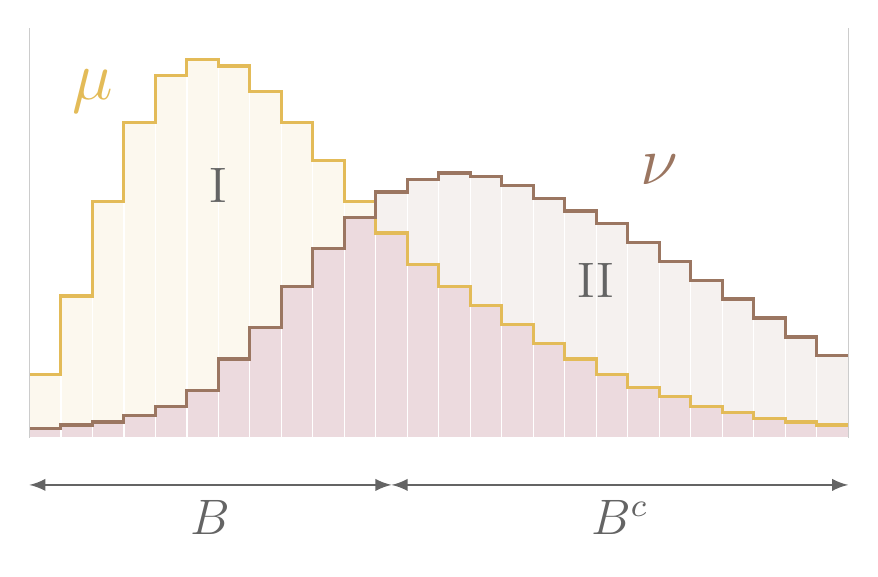
\begin{tikzpicture}[xscale=0.4, yscale=0.4, font=\large]
        % Kolory
        \definecolor{fillPink}{RGB}{236, 218, 222}
        \definecolor{lineMu}{RGB}{227, 187, 88}
        \definecolor{lineNu}{RGB}{155, 118, 97}
        \definecolor{textGray}{RGB}{100, 100, 100}
        \colorlet{fillMu}{lineMu!10}
        \colorlet{fillNu}{lineNu!10}

        % Dane
        \def\data{
            0/  2.0/ 0.3, 1/  4.5/ 0.4, 2/  7.5/ 0.5, 3/ 10.0/ 0.7,
            4/ 11.5/ 1.0, 5/ 12.0/ 1.5, 6/ 11.8/ 2.5, 7/ 11.0/ 3.5,
            8/ 10.0/ 4.8, 9/  8.8/ 6.0, 10/ 7.5/ 7.0, 11/ 6.5/ 7.8,
            12/ 5.5/ 8.2, 13/ 4.8/ 8.4, 14/ 4.2/ 8.3, 15/ 3.6/ 8.0,
            16/ 3.0/ 7.6, 17/ 2.5/ 7.2, 18/ 2.0/ 6.8, 19/ 1.6/ 6.2,
            20/ 1.3/ 5.6, 21/ 1.0/ 5.0, 22/ 0.8/ 4.4, 23/ 0.6/ 3.8,
            24/ 0.5/ 3.2, 25/ 0.4/ 2.6
        }

        % Wypełnienie pasków
        \foreach \x/\mu/\nu in \data {
            \pgfmathsetmacro{\minH}{min(\mu,\nu)}
            \pgfmathsetmacro{\maxH}{max(\mu,\nu)}
            
            % Przecięcie
            \fill[fillPink, draw=white, line width=0.5pt] (\x, 0) rectangle (\x+1, \minH);
            
            % Różnica
            \ifdim \mu pt > \nu pt
                % Region I -> fillMu
                \fill[fillMu, draw=white, line width=0.5pt] (\x, \minH) rectangle (\x+1, \maxH);
            \else
                % Region II -> fillNu
                \fill[fillNu, draw=white, line width=0.5pt] (\x, \minH) rectangle (\x+1, \maxH);
            \fi
        }

        \newcommand{\muPath}{} \newcommand{\nuPath}{}
        \foreach \x/\mu/\nu [count=\i] in \data {
            \ifnum\i=1
                \xdef\muPath{(\x,\mu) -- (\x+1,\mu)}
                \xdef\nuPath{(\x,\nu) -- (\x+1,\nu)}
            \else
                \xdef\muPath{\muPath -- (\x,\mu) -- (\x+1,\mu)}
                \xdef\nuPath{\nuPath -- (\x,\nu) -- (\x+1,\nu)}
            \fi
        }
        \draw[lineMu, very thick] \muPath;
        \draw[lineNu, very thick] \nuPath;

        \draw[gray!40] (0,0) -- (0, 13);
        \draw[gray!40] (26,0) -- (26, 13);

        \node[lineMu] at (2, 11) {\Huge $\mu$};
        \node[lineNu] at (20, 8.5) {\Huge $\nu$};
        \node[textGray, scale=1.5] at (6, 8) {I};
        \node[textGray, scale=1.5] at (18, 5) {II};

        \draw[<->, >=latex, line width=1pt, textGray] (0, -1.5) -- (11.5, -1.5) 
            node[midway, below, scale=1.5] {$B$};
        \draw[<->, >=latex, line width=1pt, textGray] (11.5, -1.5) -- (26, -1.5) 
            node[midway, below, scale=1.5] {$B^c$};
    \end{tikzpicture}
	\end{center}
	
	Wiemy, że pole pod \(\mu = 1\) oraz pole pod \(\nu = 1\). W takim razie, możemy zauważyć że pola I i II są sobie wzajemnie równe. Dodatkowo, patrząc na definicję normy całkowitego wahania, można prosto zauważyć, że jest ona równa polu I (bo B to zbiór w którym \(\mu\) najbardziej dominuje nad \(\nu\)) oraz polu II (analogicznie). Prosto widzimy, że
	\[
		\text{Pole I} = \mu(B) - \nu(B)
	\]
	\[
		\text{Pole II} = \nu(B^c) - \mu(B^c)
	\]
	Co kończy dowód
\end{proof}
%</probabil-2025-11-21-norma-calkowitego-wahania>

\begin{lemma}
	Niech \(\mu, \nu\) będą rozkładami prawdopodobieństwa nad skończonym zbiorem \(S\). Zachodzi
	\[ \left\|\mu-\nu\right\|_{TV} = \frac{1}{2} \sum_{x \in S}^{} \left|\mu\left( x  \right) - \nu\left( x \right) \right| .\]
\end{lemma}
\begin{proof}
	Z poprzedniego lematu dostajemy, że dla \(B = \left\{ x \in  S : \mu\left( x  \right) \ge \nu\left( x \right)  \right\} \) jest
	\[ \left\|\mu-\nu\right\|_{TV} = \frac{1}{2} \left( \mu\left( B  \right) - \nu\left( B  \right) + \nu\left( B^{c} \right) - \mu\left( B^{c} \right)  \right) = \frac{1}{2} \sum_{x \in S}^{} \left|\mu\left( x  \right) - \nu\left( x  \right) \right|. \]
\end{proof}

\begin{lemma}
	Niech \(\mu, \nu\) będą rozkładami prawdopodobieństwa nad skończonym zbiorem \(S\). Zachodzi
	\[ \left\|\mu-\nu\right\|_{TV} = \frac{1}{2} \sup \left\{ \sum_{x \in  S}^{} f\left( x  \right) \mu\left( x  \right) - \sum_{x \in  S}^{} f\left( x  \right) \nu\left( x  \right) : \max_{x \in S}\left|f\left( x  \right) \right|\le 1 \right\}  .\]
\end{lemma}
\begin{proof}
	\(\left( \ge  \right) \) Jeśli \(\max_{x \in S }\left|f\left( x  \right) \right|\le 1\), to mamy
	\begin{align*}
		\frac{1}{2} \left|\sum_{x \in  S}^{} f\left( x  \right) \mu\left( x  \right) - \sum_{x \in  S}^{} f\left( x  \right) \nu\left( x  \right) \right| & \le  \frac{1}{2} \sum_{x \in S}^{} \left|f\left( x  \right) \left( \mu\left( x  \right) - \nu\left( x  \right)  \right) \right| \\
		                                                                                                                                                  & \le  \frac{1}{2} \sum_{x \in S}^{} \left|\mu\left( x  \right) - \nu\left( x  \right) \right| = \left\|\mu-\nu\right\|_{TV}.
	\end{align*}

	\(\left( \le  \right) \) Bierzemy \(B = \left\{ x \in S : \mu\left( x  \right) \ge \nu\left( x \right)  \right\} \) i definiujemy funkcję
	\[ f^{\star}\left( x  \right)  = \left\{ \begin{array}{lr} 1, & x \in B \\ -1, & x \in B^{c} \end{array} \right. , \]
	która daje
	\[ \frac{1}{2} \left( \sum_{x \in S}^{} f^{\star}\left( x  \right) \mu\left( x  \right) - \sum_{x \in S}^{} f^{\star}\left( x  \right) \nu\left( x  \right)  \right) = \frac{1}{2} \sum_{x \in S}^{} \left|\mu\left( x  \right) - \nu\left( x  \right) \right|= \left\|\mu-\nu\right\|_{TV}. \]
\end{proof}

\begin{definition}
	Niech \(\mu, \nu\) będą rozkładami prawdopodobieństwa nad skończonym zbiorem \(S\). Sprzęganiem \(\mu\) i \(\nu\) nazywamy dowolną parę zmiennych losowych \(\left( X,Y \right) \) taką, że \(X\) ma rozkład \(\mu\), a \(Y\) ma rozkład \(\nu\). W szczególności te zmienne nie muszą być niezależne.
\end{definition}

\begin{lemma}
	Niech \(\left( X,Y \right) \) będzie sprzęganiem \(\mu\) i \(\nu\). Zachodzi
	\[ \left\|\mu-\nu\right\|_{TV} \le P\left( X \neq Y \right) . \]
	Ponadto istnieje sprzęganie dla którego zachodzi równość.
\end{lemma}
\begin{proof}
	Dla dowolnego \(A \subseteq S\) mamy
	\[ \mu\left( A  \right) - \nu\left( A  \right) = P\left( X \in A  \right) - P\left( Y \in  A  \right) \le P\left( X \in A \cap Y \notin A  \right) \le P \left( X \neq Y \right) . \]
	Analogicznie \(\nu\left( A  \right) - \mu\left( A  \right) \le  P\left( X \neq Y \right) \). To daje żądaną nierówność.

	Teraz skonstruujemy sprzęganie spełniające równość. Niech \(B = \left\{ x \in S : \mu\left( x  \right) \ge \nu\left( x  \right)  \right\} \). Niech \(p_1 = \mu\left( B  \right) - \nu\left( B  \right) \), \(p_2 = \nu\left( B^{c} \right) - \mu\left( B^{c} \right) \). Mamy \(p_1 = p_2 = \left\|\mu-\nu\right\|_{TV}\). Niech \(p_3 = 1-p_1 = 1-p_2\).

	Rzucamy monetą z prawdopodobieństwem orła \(p_3\). Jeśli wypadnie orzeł to ustalamy \(X = Y = s \), gdzie \(s\) wybieramy z \(S\) z rozkładem \(\left( \frac{1}{p_3} \min\left( \mu\left( s  \right) ,\nu\left( s  \right)  \right) : s \in S \right) \). Jeśli wypadnie reszka ustalamy \(X = x \) i \(Y=y\), gdzie \(x\) jest wybierany losowo z \(S \) z rozkładem \(\left( \frac{1}{p_1} \max\left( \mu\left( x  \right) -\nu\left( x  \right) , 0 \right) : x \in S \right) \), a \(y\) z rozkładem \(\left( \frac{1}{p_2} \max\left( \nu\left( x  \right) -\mu\left( x  \right) , 0 \right) : x \in S \right) \). W przypadku reszki jedna zmienna przyjmuje tylko te wartości, na których \(\mu\) jest większe, a druga tylko te, na których \(\nu\) jest większe. Mamy więc \(P\left( X\neq Y \right) = 1-p_3 = \left\|\mu-\nu\right\|_{TV}\), a \(\left( X,Y \right) \) faktycznie jest sprzęganiem \(\mu\) i \(\nu\) -- zmienne mają odpowiednie rozkłady.
\end{proof}

